It can be argued, that superconducting correlations are not possible in thin wires due to the presence of fluctuations. However in real systems this difficulty can be avoided with the help of the proximity effect. The wire itself is assumed to be metallic or semiconducting, and being put close to a strong superconductor. Due to proximity effect it's possible to obtain a presence of order parameter inside initially nonsuperconducting wire. 

\begin{figure}
	\centering
	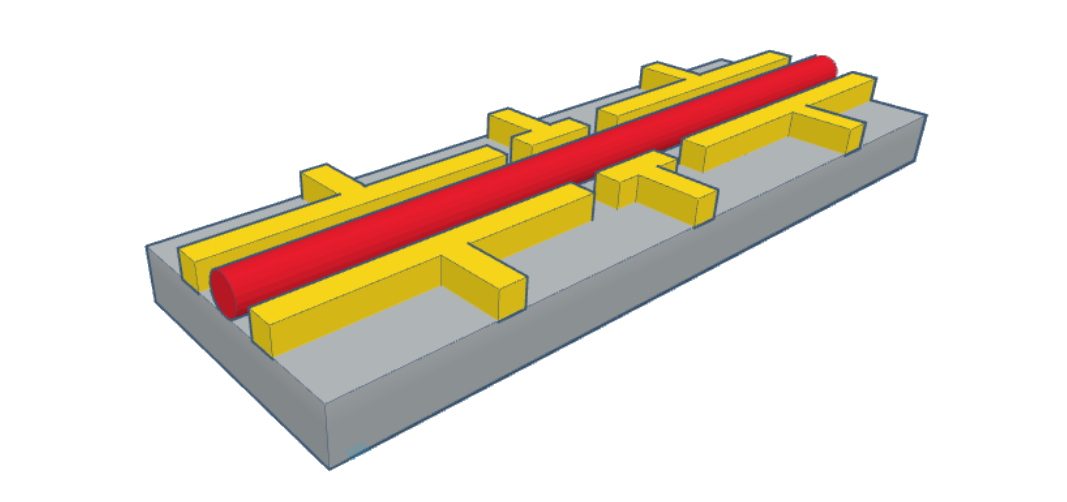
\includegraphics[width=0.7\linewidth]{images/like_real}
	\caption{Possible experimental realization of the system. The red is a metallic or semiconducting wire, the yellow are the gates and the gray is a proximitized superconductor }
	\label{fig:likereal}
\end{figure}

Taking into account the problem statement from this chapter, one can imagine the system to be like the one presented on figure \ref{fig:likereal} -- a wire put near the superconductor and equipped with a set of gates altering chemical potential. There were attempts \cite{quintized_conductance_Zhang} to create sample close to this and look for the signatures of the Majorana fermion there. 
